% Hand-authored TikZ. Workspace "thought" visualization in the style of the
% Jacobian-lens slice view: a layer x token grid whose cell shading is the
% lens read-out negentropy from gate L7 (band articulation), with an
% entropy-gated write event and its band-targeted readback annotated. This is
% the paper-static analogue of the interactive trace players in apps/web.
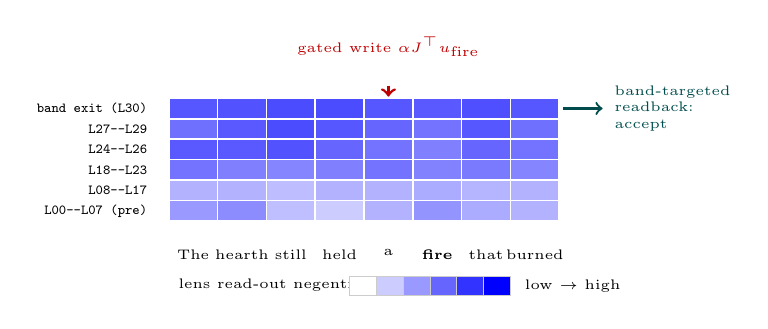
\begin{tikzpicture}[font=\scriptsize]
\def\cw{0.62}   % cell width
\def\ch{0.26}   % cell height
% negentropy by layer (gate L7 jacobian_lens.per_layer_negentropy, subsampled
% to the eight decode positions shown); higher = brighter band read-out.
% columns = decode tokens; rows = layer bands (early -> workspace band exit)
% each row is a layer group; shading value in [0,1] from the L7 array.
\foreach \r/\lab/\vals in {
  6/{band exit (L30)}/{0.66,0.68,0.70,0.70,0.66,0.65,0.69,0.66},
  5/{L27--L29}/{0.56,0.65,0.70,0.66,0.60,0.55,0.66,0.56},
  4/{L24--L26}/{0.65,0.65,0.68,0.60,0.55,0.50,0.60,0.55},
  3/{L18--L23}/{0.55,0.50,0.48,0.50,0.55,0.49,0.52,0.48},
  2/{L08--L17}/{0.30,0.30,0.26,0.30,0.30,0.33,0.29,0.30},
  1/{L00--L07 (pre)}/{0.40,0.45,0.25,0.20,0.30,0.42,0.33,0.30}}{
  \foreach \c/\v in {0/\vals} {}
  \pgfmathsetmacro{\y}{\r*\ch}
  \node[anchor=east, font=\tiny\ttfamily] at (-0.15,\y+0.5*\ch) {\lab};
  \foreach \c [count=\ci from 0] in \vals {
    \pgfmathsetmacro{\x}{\ci*\cw}
    \pgfmathsetmacro{\shade}{100*\c}
    \fill[blue!\shade!white, draw=white, line width=0.6pt]
      (\x,\y) rectangle (\x+\cw,\y+\ch);
  }
}
% token labels along the bottom (a representative gated fire-case decode)
\foreach \c/\tok [count=\ci from 0] in {0/The,1/hearth,2/still,3/held,4/a,5/{\bf fire},6/that,7/burned} {
  \pgfmathsetmacro{\x}{\ci*\cw + 0.5*\cw}
  \node[anchor=north, font=\tiny] at (\x,0.02) {\tok};
}
% write event (sphuratta gate) at the high-entropy step before "fire"
\draw[->, red!75!black, line width=1pt]
  (4.5*\cw,6*\ch+0.42) -- (4.5*\cw,6*\ch+\ch+0.02);
\node[red!75!black, font=\tiny, anchor=south] at (4.5*\cw,6*\ch+\ch+0.40)
  {gated write $\alpha J^{\top}u_{\mathrm{fire}}$};
% readback annotation at the band exit
\draw[->, teal!60!black, line width=0.8pt]
  (8*\cw+0.05,6*\ch+0.5*\ch) -- (8*\cw+0.55,6*\ch+0.5*\ch);
\node[teal!60!black, font=\tiny, anchor=west, align=left]
  at (8*\cw+0.58,6*\ch+0.5*\ch) {band-targeted\\readback:\\accept};
% colour key
\node[font=\tiny, anchor=west] at (0,-0.55) {lens read-out negentropy:};
\foreach \i in {0,...,5} {
  \pgfmathsetmacro{\sh}{20*\i}
  \pgfmathsetmacro{\x}{2.3+\i*0.34}
  \fill[blue!\sh!white, draw=gray!40] (\x,-0.68) rectangle (\x+0.34,-0.44);
}
\node[font=\tiny, anchor=west] at (4.4,-0.56) {low $\rightarrow$ high};
\end{tikzpicture}
